\begin{frame}{Processing IACT data}
    \centering
    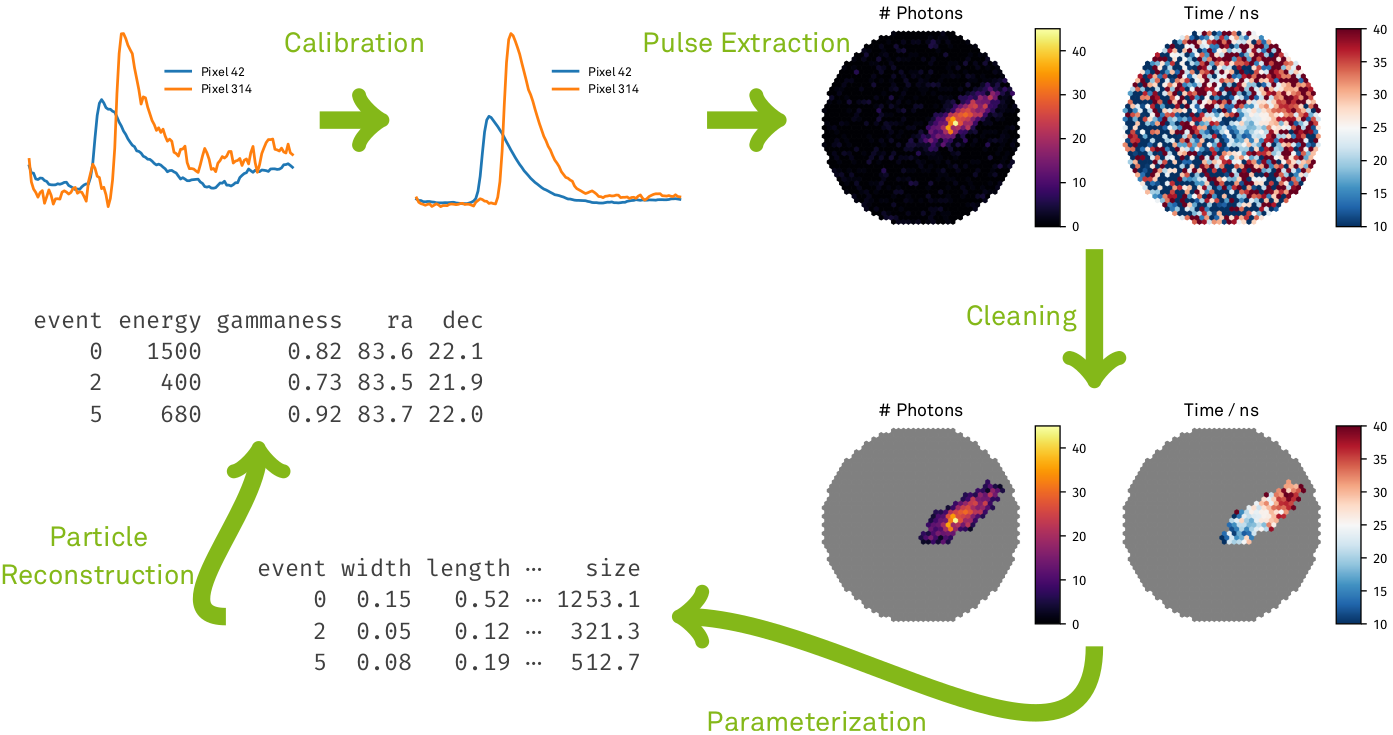
\includegraphics[width=0.9\textwidth]{images/prepro.png}\\[-1.25\baselineskip]
    \hspace{11cm}\href{https://github.com/MaxNoe/phd_thesis}{[Max Noethe, PhD thesis]}

    \note[item]{Rohdaten = Spannungskurven pro Pixel}
    \note[item]{Kurven bereinigt}
    \note[item]{Integration Photonenladung \& Ankunftszeit (Hälfte der Photonenladung)}
    \note[item]{Pixel ohne Signal entfernen}
    \note[item]{Parameter berechnen}
    \note[item]{Rekonstruktion phy. Eigenschaften (meine Arbeit)}
\end{frame}

\begin{frame}{Image features}
    \begin{columns}[onlytextwidth]
        \begin{column}{0.475\textwidth}
            \begin{itemize}
                \item Hillas Parameters
                    \begin{itemize}
                        \item PCA of the integrated photon charge
                        \item Position of center of gravity
                        \item Angle of main shower axis
                        \item \texttt{length}, \texttt{width}: standard deviations
                        \item[\textbf{\textcolor{tugreen}{\to}}] Describe extent of shower
                    \end{itemize}
                \item Timing parameters based on arrival times
                    \begin{align*}
                        y = \mathtt{time\_gradient} \cdot x + \mathtt{intercept}
                    \end{align*}
                \item \texttt{leakage} parameters describe amount of light in outermost pixels
                \item \texttt{intensity} describes total amount of light in shower
                \item and others...
            \end{itemize}
        \end{column}
        \begin{column}{0.475\textwidth}
            \centering
            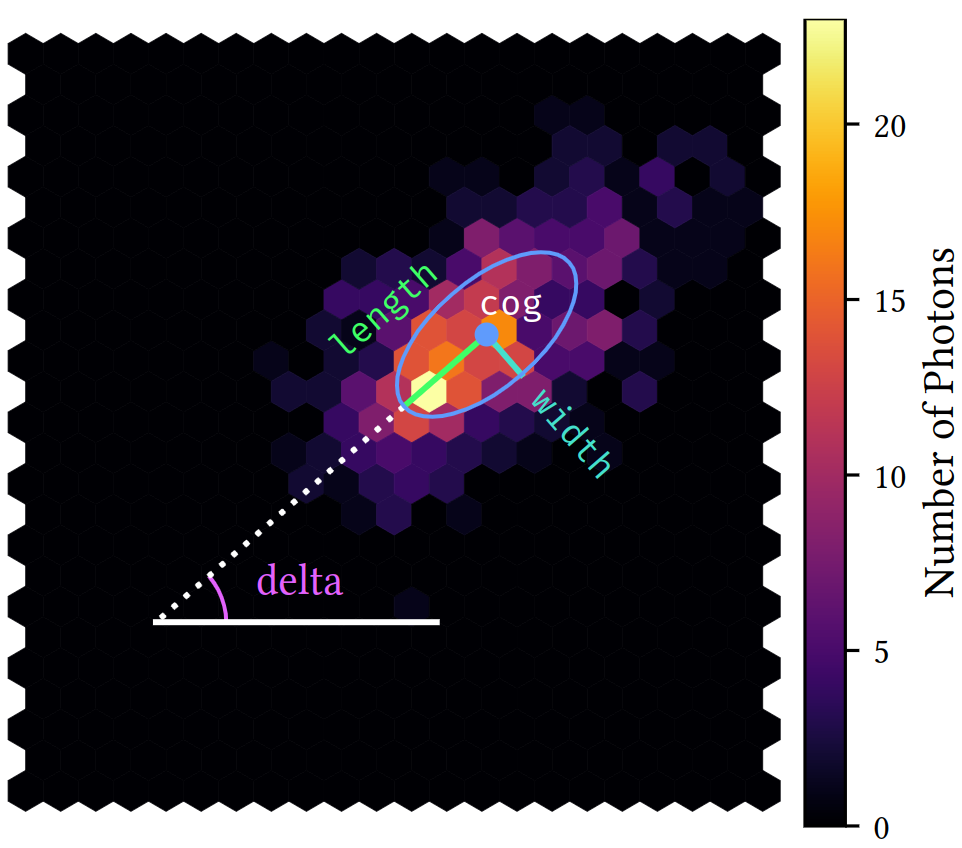
\includegraphics[width=\textwidth]{images/hillas.png}\\[-0.5\baselineskip]
            \hspace{1.5cm}\href{https://github.com/MaxNoe/phd_thesis}{[Max Noethe, PhD thesis]}
        \end{column}
    \end{columns}

    \note[item]{Wichtige Bildparameter}
    \note[item]{Hillas P. $\to$ Hauptkomponentenanalyse Photonenladung
        \newline - Position Schwerpunkt Verteilung 
        \newline - Orientierung Hauptachse
        \newline - \texttt{length}, \texttt{width} = Standartabweichungen entlang Hauptkomponenten 
        \newline (- 3tes, 4tes Moment auch berechnet)
        \newline $\to$ Beschreiben Ausdehnung und Position
    }
    \note[item]{Lineare Regression entlang Hauptachse anhand Ankunftszeiten}
    \note[item]{\texttt{leakage} beschreiben Licht am Rand $\to$ Wie viel vlt. nicht von Kamera aufgezeichnet}
    \note[item]{\texttt{intensity} = Licht insgesamt in Kamera}
\end{frame}

\begin{frame}{Data used}
    \begin{itemize}
        \item<1-> Monte Carlo Simulatons: point-source gamma-rays, diffuse gamma-rays, diffuse protons
        \item<1-> Crab Nelua observation
            \begin{itemize}
                \item 18th January, 2020
                \item \SI{2.6}{\hour} target observation and \SI{1.3}{\hour} off region observation
            \end{itemize}
        \item<1-> Markarian 421 observation
            \begin{itemize}
                \item 20th June, 2020
                \item \SI{2.2}{\hour} wobble mode observation
            \end{itemize}
    \end{itemize}
    \medskip
    \onslide<2->{
        Processed up to image parameter level: lstchain
        \begin{itemize}
            \item v0.5.1
            \item v0.5.2 $\to$ among others: scaling of optical efficiency of camera (observed efficiency = \sfrac{2}{3} simulated efficiency) 
        \end{itemize}
    }

    \note<1->[item]{Gamma Astronomie $\to$ Detektorverhalten mit Simulationen 
        \newline da keine Photonen mit so hohen Energien im Labor
        \newline Hier Gamma von Punktquelle, diffuse Gammas, diffuse Protonen $\to$ Training
    }
    \note<1->[item]{Modelle angewendet $\to$ Observationsdaten Krebsnebel und AGN Marakrian 421}
    \note<1->[item]{Krebs: - 18.1.2020 
        \newline - ON/OFF 
    }
    \note<1->[item]{Mrk 421: - 20.6.2020 
        \newline - wobble mode
    }
    \note<2->[item]{Daten vorbereitet bis Bildparameter lvl $\to$ lstchain}
    \note<2->[item]{MCs $\to$ 2 Versionen $\to$ verglichen
        \newline - v0.5.2 im Laufe der Arbeit released
        \newline - da (Mitglieder LST Kollaboration) optische Eff. nur \sfrac{2}{3} $\to$ Skalierung in lstchain
    }
\end{frame}
